%===============================================================================
% ifacconf.tex 2022-02-11 jpuente  
% Template for IFAC meeting papers
% Copyright (c) 2022 International Federation of Automatic Control
%===============================================================================
\documentclass{ifacconf}

\usepackage{graphicx}      % include this line if your document contains figures
\usepackage{natbib}        % required for bibliography
\usepackage{hyperref}	   % required for hyperlinks
\usepackage{amssymb}	   % symbol for therefore dots
\usepackage{comment}	   % Package for multi-line commenting
%===============================================================================
\begin{document}
\begin{frontmatter}

\title{Trends in the Development of AI for Games\thanksref{footnoteinfo}}
% Title, preferably not more than 10 words.

\thanks[footnoteinfo]{This research was carried out in collaboration with the INSYTE-Cooley Research Laboratory, SETU, Ireland and with and the support of the Dept. Computing and Mathematics, SETU.}

\author[First]{Patrick McInerney} 
\author[Second]{Brendan Lyng} 

\address[First]{Dept. Computing and Mathematics, SETU, Ireland (e-mail: patrick.mcinerney@setu.ie)}
\address[Second]{Dept. Computing and Mathematics, SETU, Ireland (e-mail: brendn.lyng@setu.ie)}

\begin{abstract}                % Abstract of not more than 250 words.
Abstract text here
\end{abstract}

\begin{keyword}
Artificial intelligence, games.
\end{keyword}

\end{frontmatter}
%===============================================================================
% \begin{comment}

\section{Bits and Bobs}

Statement for Citation Type 1: So on and so forth \citep{Morris:2022}.
 
Statement for Citation Type 2: \cite{Garca2018} states so on and so forth. 

Statement for Citation Type 3: So on and so forth \citep*{CDWA}.

Italics: 'preventative \textit{conservation}'.

Degree symbol: 57.4$^\circ$.

Percent symbol: 18\%

Numbered list:

\begin{enumerate}
	\item Item 1
	\item Item 2
	\item Item 3
\end{enumerate}

\begin{figure}
	\begin{center}
		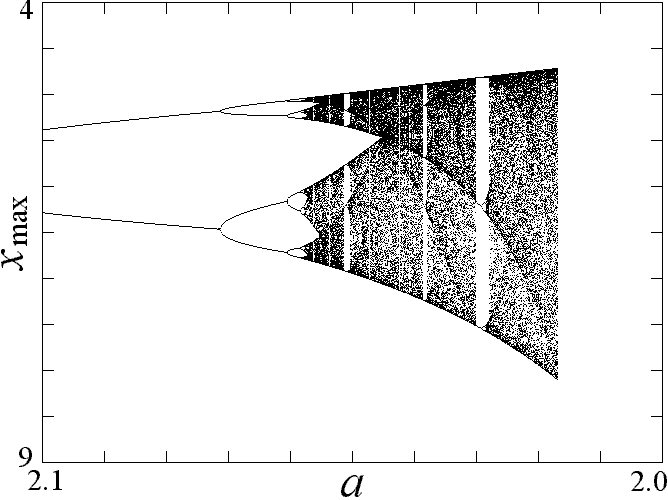
\includegraphics[width=8.4cm]{bifurcation}    % The printed column width is 8.4 cm.
		\caption{Some image here} 
		\label{fig:my_fig1}
	\end{center}
\end{figure}

Text format: eg Tag Image File Format (\texttt{.tiff})

For Web addresses:eg  Arches -- \url{https://www.archesproject.org/} -- is an open source Linux-based framework.

Referencing Images: See fig \ref{fig:my_fig1}

\subsubsection{Sub-Section}Sub-section text here.

\subsubsection{Sub-section}Sub-section text here.
%\end{comment}

\section{Introductionn}

Some introduction text here.

\section{Another Section}
Section text here.

\section{Another Section}

Another text block subsection here.

\section{Conclusion}

Conclusion text here.

\begin{ack}
This research was carried out in conjunction with the Dept. Computing and Mathematics.
\end{ack}

\bibliographystyle{ifacconf}
\bibliography{ifacconf}             

\end{document}
